\documentclass[a4paper,12pt]{article} 
\usepackage{mathrsfs}
\usepackage[utf8]{inputenc}
\usepackage[spanish]{babel}
\usepackage{amsmath}
\usepackage{amsfonts}
\usepackage{amssymb} 
\usepackage{graphicx} 
\usepackage{hyperref} 
\usepackage{wrapfig}
\usepackage{enumitem}
\usepackage{fancyhdr}
\usepackage{float}
\usepackage{eurosym}
\usepackage{color}
\usepackage{circuitikz}
\usepackage{titling}
\usepackage{hyperref}
\usepackage{media9}
\usepackage{lipsum}
\usepackage{tocbibind}
\usepackage{listings}
\usepackage{tabularx}
\usepackage{tcolorbox}
\usepackage{bookmark}
\usepackage{media9}
\usepackage[table]{xcolor}
\definecolor{lightblue}{RGB}{228, 244, 253}
\usepackage{listings}
\usepackage{color}

\definecolor{dkgreen}{rgb}{0,0.6,0}
\definecolor{gray}{rgb}{0.5,0.5,0.5}
\definecolor{mauve}{rgb}{0.58,0,0.82}

\lstset{frame=tb,
  language=Python,
  inputencoding=utf8,
  extendedchars=true,
  aboveskip=3mm,
  belowskip=3mm,
  showstringspaces=false,
  columns=flexible,
  basicstyle={\small\ttfamily},
  numbers=none,
  numberstyle=\tiny\color{gray},
  keywordstyle=\color{blue},
  commentstyle=\color{dkgreen},
  stringstyle=\color{mauve},
  breaklines=true,
  breakatwhitespace=true,
  tabsize=3,
  literate=%
    {á}{{\'a}}1
    {é}{{\'e}}1
    {í}{{\'i}}1
    {ó}{{\'o}}1
    {ú}{{\'u}}1
    {ñ}{{\~n}}1
    {č}{{\v{c}}}1
}
\usepackage[left=3cm,right=3cm,top=3cm,bottom=4cm]{geometry}
\sloppy

\pagestyle{fancy}
\providecommand{\abs}[1]{\lvert#1\rvert}
\providecommand{\norm}[1]{\lVert#1\rVert}

%%% Para las cabeceras
\newcommand{\hsp}{\hspace{20pt}}
\newcommand{\HRule}{\rule{\linewidth}{0.5mm}}
\headheight=50pt
%%% 
\newcommand{\vacio}{\textcolor{white}{ .}}

%%% Para que las ecuaciones se numeren
%%% con el número de sección y el de ecuación.
\renewcommand{\theequation}{\thesection.\arabic{equation}}


% Color azul para algunos 
% textos de la portada
\definecolor{azulportada}{rgb}{0.16, 0.32, 0.75}

%%%% Azul para textos de headings
\definecolor{azulinterior}{rgb}{0.0, 0.2, 0.6}

%%%%%%%%%%%%%%%%%%%%%%%%%%%%%%%%
%%%%%% Datos del proyecto %%%%%%
%%%%%%%%%%%%%%%%%%%%%%%%%%%%%%%%
%%%TÍTULO
%%% Escribirlo en minúsculas, el programa
%%% lo pondrá en mayúsculas en la portada.

\title{Calibración de la cámara}

%%%% AUTORES
\author{Lydia Ruiz Martínez \and Pablo Tuñón Laguna}

%%%%%%%%%%%%%%%%%%%%%
%%%%%%%%%%%%%%%%%%%%
\begin{document}

%%%%%%%%%%%%%%%%%%%%%%%%%%%%%%%
%%%%%%%%%%%%%%%%%%%%%%%%%%%%%%%
\begin{titlepage} %%%%% Aquí no hay que tocar nada.
	%%%% Las siguientes instrucciones generarán automáticamente
	%%%% la portada de tu proyecto.
	%%% Cambio de la estructura de esta página
\newgeometry{left=0.6cm,top=1.3cm,bottom=1.2cm}

\fbox{\parbox[c]{18.5cm}{
\begin{center}
\vspace{1.5cm}
{\fontfamily{ptm}\fontsize{24}{28.8}\selectfont{Universidad Pontificia de Comillas}}\\
[3.5em]
{\fontfamily{ptm}\fontsize{24}{5}\selectfont{ICAI}}\\
[4.5em]
{\fontfamily{ptm}\fontsize{28}{5}\selectfont{LABORATORIO 1}}\\
[2cm]
{\fontfamily{ptm}\fontsize{24}{5}\selectfont{Visión por Ordenador I}}\\
[2cm]

% Autor del trabajo de investigación
\textcolor{azulportada}{\fontfamily{ptm}\fontsize{16}{5}\selectfont{\theauthor}}\\
[2cm]
% Título del trabajo
\textcolor{azulportada}
{\fontfamily{ptm}\fontsize{30}{5}\selectfont{\textsc{\thetitle}}}\\
%{\Huge\textbf{\thetitle}}\\
[1.2cm]

\includegraphics[width=10cm]{fonts/Logo ICAI.png}
\\[1.8cm]

{\fontfamily{ptm}\fontsize{16}{5}\selectfont{Curso 2024-2025}}\\
[4cm]
\end{center}
}}
\end{titlepage}
 
 \restoregeometry
 %%%% Volvemos a la estructura de la página normal

%%%%%%%%%%%%%%%%%%%%%%%%%%%%%%

{%\Large

%%%Encabezamiento y pie de página
%%% También se genera automáticamente
%%% Mejor no tocarlo mucho.
\renewcommand{\headrulewidth}{0.5pt}
\fancyhead[R]{
	\textcolor{azulinterior}{\fontfamily{ptm}\fontsize{14}{4}\selectfont{\textbf{\thetitle}}}\\
\textcolor{azulportada}{\fontfamily{ptm}\fontsize{10}{3}\selectfont{Laboratorio 1 de Visión por Ordenador I}}\\
{\fontfamily{ptm}\fontsize{10}{3}\selectfont{\theauthor}}}
\fancyhead[L]{\vacio}

\pagestyle{fancy}
\renewcommand{\footrulewidth}{0.5pt}
\fancyfoot[L]{\footnotesize Universidad Pontificia de Comillas (ICAI) --- curso 2023-2024}
\fancyfoot[C]{\vacio}
\fancyfoot[R]{\footnotesize Página \thepage}

%%%%%%%%%%%%%%%%%%%%
\newpage

\tableofcontents

\newpage


\newpage


\section{Introducción}


\vspace{1cm}

La visión por ordenador es un campo de la computación en el cual se desarrollan algoritmos y métodos que permiten a un ordenador obtener información de las matrices de píxeles que componen una imagen.

\vspace{0.5cm}

Un ordenador no procesa del mismo modo que un cerebro humano, a no ser que se le indique, no suele ser capaz de alcanzar conclusiones de forma autónoma. Es por ello que aunque se le proporcione una imagen como un tensor, este no es capaz de identificar más que un conjunto de valores. Con algoritmos de visión por ordenador se puede calibrar una cámara para obtener sus parámetros intrínsecos (distancia focal y centro de la imagen) de tal manera que se puedan realizar cálculos de posición sobre los números que identifican los píxeles. De esta manera se pueden extraer ``features" (características) de las imágenes. La identificación de elementos en una imagen es bastante útil en el mundo moderno ya que entre algunas de sus aplicaciones destaca el entrenamiento de modelos de aprendizaje automático o el control de computacional a través de patrones de movimiento.

\vspace{0.5cm}

A lo largo del siguiente escrito se va a detallar la implementación en Python\footnote{El proyecto se ha desarrollado con un notebook (lab\_1.ipynb) para un estudio exploratorio inicial. Posteriormente, se migró a un archivo Python (CalibrateCamera.py) más estructurado para facilitar su reutilización en futuros proyectos.}
 usando la librería opencv del ajuste de un sistema estereoscópico de cámaras planas así como la corrección de una imagen tomada con ojo de pez.
 


\newpage


\section{Calibración de cámara}


\vspace{1.cm}

Para calibrar una cámara hay que tomar una serie de fotos a un entramado de cuadrados blancos y negros, modificando tanto el ángulo y la localización. En este apartado se van a tratar los pasos realizados para el ajuste y calibrado de una cámara. Desde la localización de esquinas, el ajuste de las mismas hasta la obtención de los parámetros intrínsecos de la cámara así como los extrínsecos de la imagen y los errores en el ajuste. Así mismo se estudiará el número mínimo de imágenes necesarias para calibrar una cámara y obtener un resultado preciso.

\vspace{0.5cm}

\subsection{Extracción de intersecciones}

\vspace{0.5cm}

Con las fotos tomadas y cargadas en el programa mediante \textit{imgeio.imread} (a partir de sus direcciones) se cuenta con una lista de matrices para cada una de las imágenes. El siguiente paso consiste en localizar todas las intersecciones internas de la cuadrícula fotografiada, para ello se usa la función ``findChessboardCorners" que recibe tanto las matrices correspondientes con la imagen como el tamaño de la cuadrícula interna.

\vspace{0.5cm}

La función devuelve una tupla por cada imagen, el primer valor es un booleano que indica si se han encontrado las intersecciones de la cuadrícula, el segundo valor son las coordenadas de las intersecciones encontratadas. En caso de que no se encuentren las intersecciones este elemeneto consistiría en una lista vacía. Los casos en los que no se detectan los bordes son mayoritariamente 2, si están muy borrosas o si se encuentran muy cerca del extremo de la imagen. En el caso de los datos proporcionados, en el conjunto de imágenes de la cámara derecha falla la primera foto y en las de la izquierda la decimocuarta.

\vspace{0.5cm}

\subsubsection{Mejora de intersecciones (Pregunta A2)}

Es posible mejorar las intersecciones ya calculadas, para ello lo primero que hay que hacer es definir unos criterios de ajuste definidos como una tupla en la que se le indica el número máximo de iteraciones a computar (en este caso 30) así como la la variación mínima en los parámetros permitida en el ajuste iterativo (definida como 0.01).

\vspace{0.5cm}

Posteriormente se transforman las imágenes a escala de grises ya que aumenta el contraste entre los cuadrados pudiendo encontrar así con mayor precisión la localización interna de las intersecciones de la cuadrícula. Para ello se usa la función \textit{cvtColor} que recibe la imagen y un parámetro que indica la paleta de colores a la que se convierte la imagen.

\vspace{0.5cm}

Finalmente se aplica la función \textit{cornerSubPix} que toma la imagen en blanco y negro, la localización de las cuadrículas original, una tupla que indica en qué rango de píxeles puede variar la intersección antigua (en este caso un máximo de 10 píxeles en cada dirección) así como una tupla que indica si se pueden usar todos los valores de todas las direcciones de variación (-1,-1 permite todos los puntos), también necesita los criterios de ajuste. El resultado de la función es un conjunto de valores que mejora la posición de las intersecciones anteriormente calculadas, tal y como se puede ver a continuación:

\vspace{0.5cm}


\begin{figure}[h!]
    \centering
    \begin{minipage}[b]{0.45\textwidth}
        \centering
        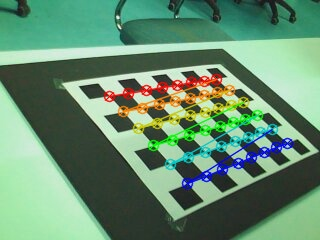
\includegraphics[width=\textwidth]{fonts/fine_0.jpg}
        \caption{Ajuste fino de intersección de cuadrícula, autoría propia.}
        \label{fig:izquierda1}
    \end{minipage}
    \hfill
    \begin{minipage}[b]{0.45\textwidth}
        \centering
        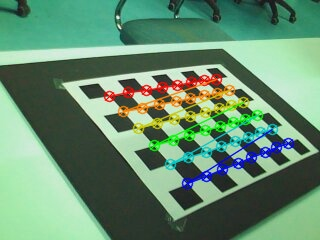
\includegraphics[width=\textwidth]{fonts/not_fine_0.jpg}
        \caption{Ajuste fino de intersección de cuadrícula, autoría propia.}
        \label{fig:derecha1}
    \end{minipage}

\end{figure}

\vspace{0.5cm}

\subsection{Obtención de parámetros}

\vspace{0.5cm}

Antes de usar la función de calibrado se necesita obtener las coordenadas de los puntos marcados con respecto a la imágen, de tal manera que el punto rojo de arriba a la izquierda es el (0, 0, 0), el punto naranja el (30, 0, 0), el segundo punto rojo (0, 30, 0) y así sucesivamente. Las variaciones son de 30 debido a que el lado de los cuadrados de la la cuadrícula mide 30 mm.

\vspace{0.5cm}

Posteriormente es necesario replicar el proceso tantas veces como imágenes se vayan a procesar y almacenar los resultados en una lista. Finalmente se procede a aplicar la función \textit{calibrateCamera} que recibe la liste mencionada, las intersecciones de cada imagen y el tamaño en píxeles de cada imagen. La aplicación de esta función devuelve la matriz de intrínsecos \textit{K}, la de extrínsecos \textit{e} (una combinación de los de rotación y traslación \ref{appendix:a}[Anexo 1]), los coeficientes de distorsión \textit{d}, y el error de ajuste \textit{rms}:

\vspace{0.5cm}

% Matriz de intrínsecos
\[
K = \begin{pmatrix}
420.334 & 0 & 149.42 \\
0 & 421.04 & 128.62 \\
0 & 0 & 1
\end{pmatrix}
\]

% Coeficientes de distorsión
\[
\mathbf{d} = \begin{pmatrix}
-2.47e-2 & -2.13 & 4.10e-3 & -6.79e-3 & 1.13e1
\end{pmatrix}
\]

% RMS
$$rms=0.09$$

\vspace{0.5cm}

\subsection{Número mínimo de imágenes necesarias para calibrar (Pregunta A3)}

\vspace{0.5cm}

Para determinar el número adecuado de imágenes para calibrar la cámara, se ha elaborado un diagrama de Pareto que ilustra la relación entre el error cuadrático medio (RMS) y el número de imágenes empleadas en la calibración. Este gráfico permite observar cómo varía el error RMS a medida que se incrementa el número de imágenes, facilitando la identificación del punto óptimo donde añadir más imágenes contribuye mínimamente a la reducción del error.

\vspace{0.5cm}

\begin{figure}[h]
    \centering
    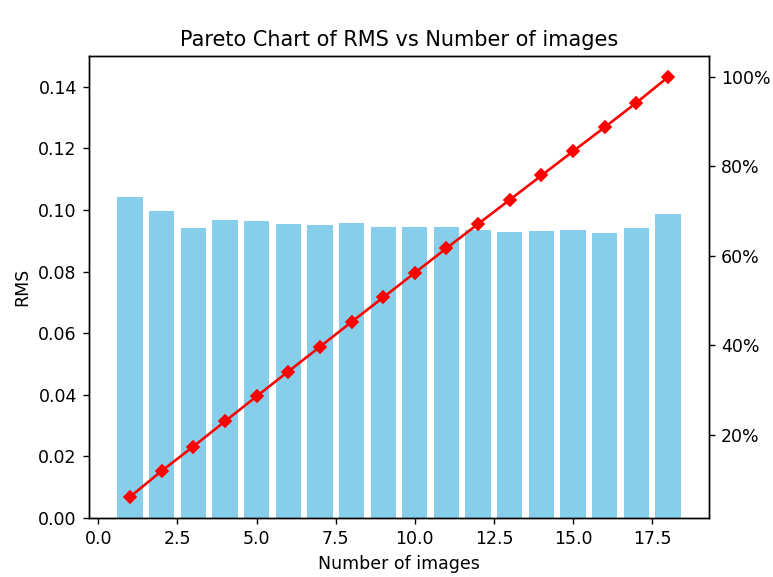
\includegraphics[width=0.6\textwidth]{fonts/pareto.png}
    \caption{Diagrama de Pareto que representa el rms de la calibración en función del número de imágenes, autoría propia}
    \label{fig:imagen}
\end{figure}

\vspace{0.5cm}

Del diagrama anterior se extrae que 3 es el número de imágenes óptimas para el calibrado de una cámara. Cabe destacar que con más imágenes el error es ligéramente mayor y aparentemente constante por lo que tampoco supone un gran problema usar un mayor número de imágenes siempre y cuando no se superen las 17 imágenes ya que el error asciende de nuevo a partir de dicho número. Sería relevante usar un dataset con imágenes recortadas, giradas y emborronadas para comparar el resultado así como reforzar la hipótesis obtenida.

\vspace{0.5cm}

\subsection{Sistema estereoscópico (Pregunta A1)}

\vspace{0.5cm}

Tal y como se explicó en la introducción del estudio, se la implementación es capaz de calibrar sistemas estereoscópicos, ya que un sistema estereoscópico no es más que un sistema con doble cámara, las cuales se pueden calibrar de forma aislada. Cabe destacar que las ventajas del uso de un sistema de estas características en lugar de una única cámara son múltiples ya que permite una mejor localización de los objetos así como eliminar los puntos muertos que puedan surgir por agentes interrumpiendo el campo visual. Hasta este instante se ha realizado una implementación para calibrar la cámara derecha, sin embargo, sustituyendo la ruta de entrada de las imágenes es posible calibrar la cámara restante del sistema. Al realizar los pasos anteriores sobre las imágenes tomadas por la cámara derecha se obtienen los siguientes coeficientes intrínsecos K, extrínsecos \textit{e} (una combinación de los de rotación y traslación \ref{appendix:a}), coeficientes de distorsión y RSM.

% Matriz de intrínsecos
\[
K = \begin{pmatrix}
429.6632 & 0 & 145.0714 \\
0 & 430.8301 & 137.6744 \\
0 & 0 & 1
\end{pmatrix}
\]

% Coeficientes de distorsión
\[
\mathbf{d} = \begin{pmatrix}
-0.1131 & -0.2395 & 0.0065 & -0.0055 & 1.6672
\end{pmatrix}
\]

% RMS
$$rms = 0.09$$

\begin{figure}[h]
    \centering
    \begin{minipage}[b]{0.45\textwidth}
        \centering
        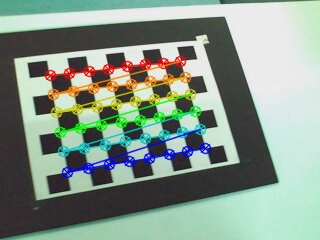
\includegraphics[width=\textwidth]{fonts/detected_17.jpg}
        \caption{Detección de intersecciones internas para la cámara derecha, imagen 17, autoría propia.}
        \label{fig:izquierda1}
    \end{minipage}
    \hfill
    \begin{minipage}[b]{0.45\textwidth}
        \centering
        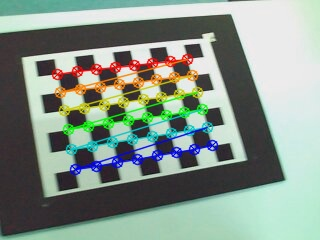
\includegraphics[width=\textwidth]{fonts/detected_18.jpg}
        \caption{Detección de intersecciones internas para la cámara derecha, imagen 18, autoría propia.}
        \label{fig:derecha1}
    \end{minipage}

\end{figure}

\newpage


\section{Corrección de Distorsión}


\vspace{1cm}

Antes de realizar la corrección de distorsión de una lente de pez se debe calibrar la cámara. Cabe destacar que el calibrado de cámara se realiza mediante el mismo proceso explicado en a lo largo del apartado anterior. Usando la implementación ya comentada se obtiene la matriz de intrínsecos $K$ así como los coeficientes de distorsión $\mathbf{d}$ y los parámetros extrínsecos (ver \ref{appendix:b}).

% Matriz de intrínsecos
\[
K = \begin{pmatrix}
188.50770041 & 0 & 504.10055382 \\
0 & 184.96088979 & 373.6659997 \\
0 & 0 & 1
\end{pmatrix}
\]

% Coeficientes de distorsión
\[
\mathbf{d} = \begin{pmatrix}
0.08230382 \\
0.00263929 \\
0.03569538 \\
-0.03186732
\end{pmatrix}
\]
\subsection{Eliminación de distorsión de imágenes (Pregunta B1)}

\vspace{0.5cm}

Para la eliminación de la distorsión se comienza usando la función \textit{initUndistortRectifyMap} para crear dos mapas de corrección basados en los parámetros de la cámara. Estos mapas definen el formato de los pixeles de la imagen principal para eliminar la transformación. 

Posteriormente se aplica la función \textit{remap} para corregir las imágenes usando los mapas generales obteniendo de esta manera imágenes con una menor distorsión, con menor curvatura así como proporciones reales restauradas.

\newpage

\begin{figure}[h!]
    \centering
    \begin{minipage}[b]{0.45\textwidth}
        \centering
        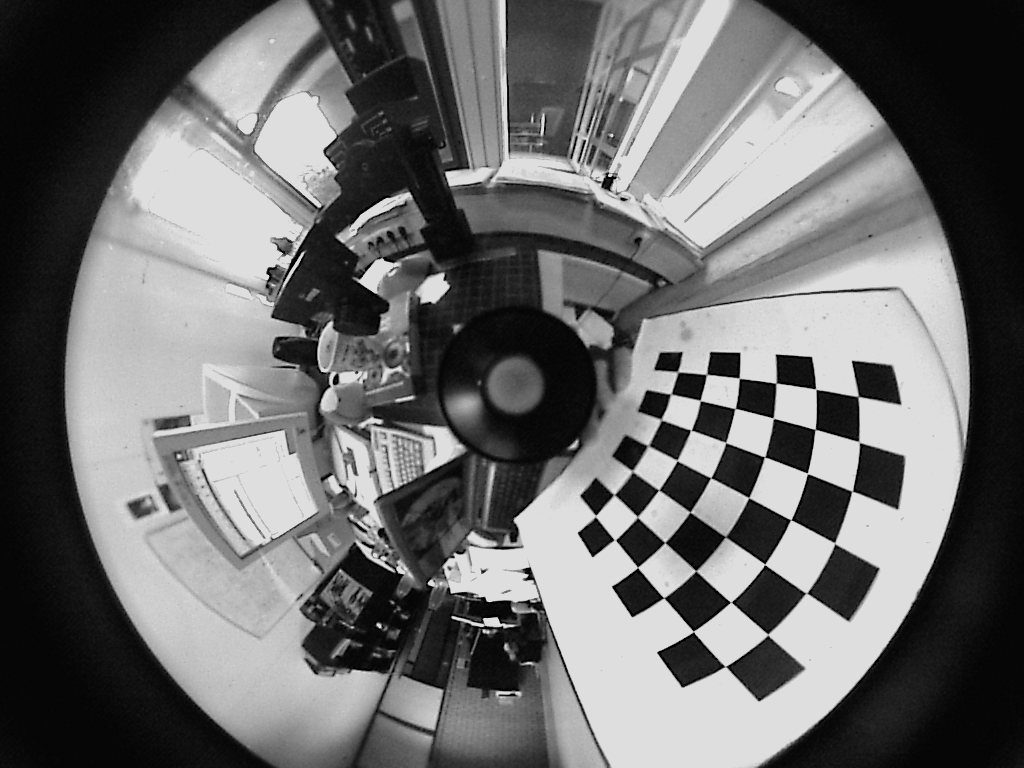
\includegraphics[width=\textwidth]{fonts/VMRImage0.jpg}
        \caption{Imagen 1 original, dataset.}
        \label{fig:izquierda1}
    \end{minipage}
    \hfill
    \begin{minipage}[b]{0.45\textwidth}
        \centering
        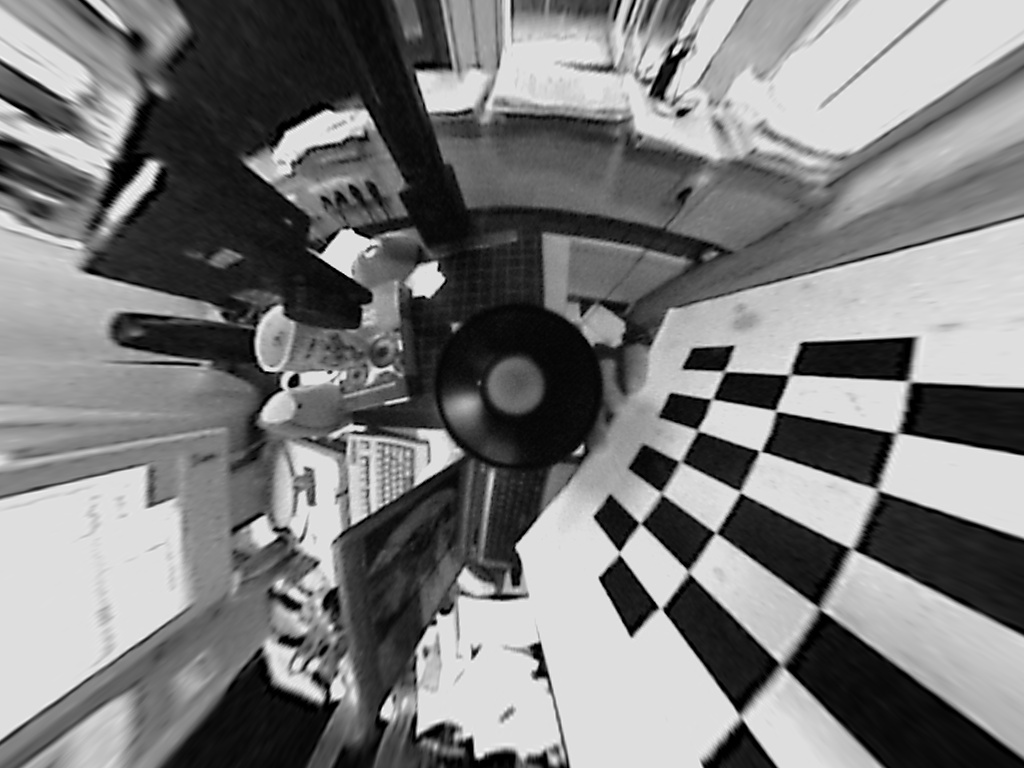
\includegraphics[width=\textwidth]{fonts/fisheye_0.jpg}
        \caption{Imagen 1 corregida, autoría propia.}
        \label{fig:derecha1}
    \end{minipage}
    
    \vspace{1cm} 

    \begin{minipage}[b]{0.45\textwidth}
        \centering
        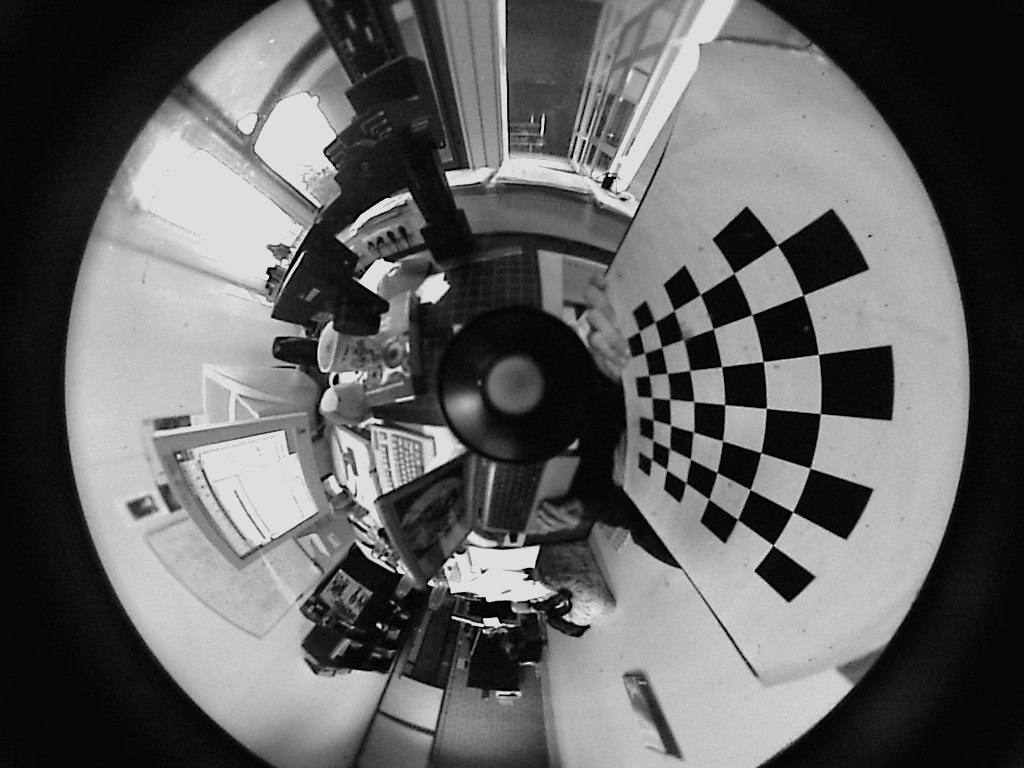
\includegraphics[width=\textwidth]{fonts/VMRImage1.jpg}
        \caption{Imagen 2 original, dataset.}
        \label{fig:izquierda2}
    \end{minipage}
    \hfill
    \begin{minipage}[b]{0.45\textwidth}
        \centering
        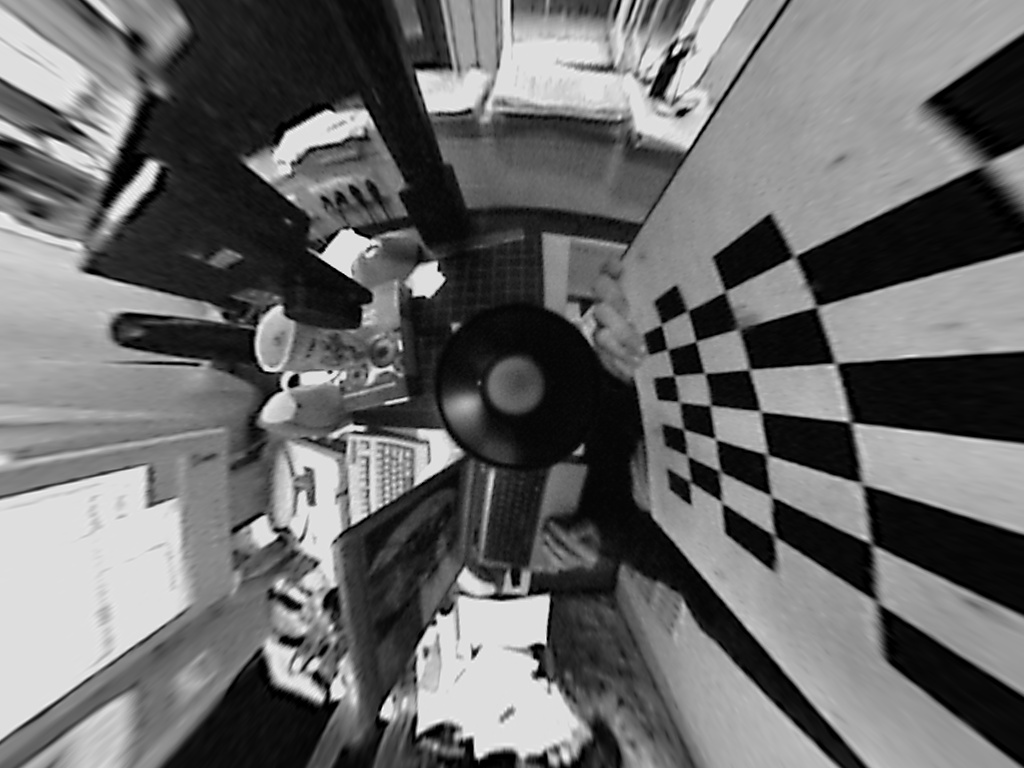
\includegraphics[width=\textwidth]{fonts/fisheye_1.jpg}
        \caption{Imagen 2 corregida, autoría propia.}
        \label{fig:derecha2}
    \end{minipage}
\end{figure} 

\newpage

\appendix


\section{Anexos}

\vspace{0.5cm}

\subsection{Parámetros extrínsecos de las imágenes derechas} \label{appendix:a}

\[
e_1 = \begin{pmatrix}
0.59 & 0.73 & 0.34 & -48.90 \\
0.65 & -0.18 & -0.74 & -39.93 \\
-0.48 & 0.66 & -0.58 & 512.10
\end{pmatrix}
\]

\[
e_2 = \begin{pmatrix}
0.58 & 0.74 & 0.35 & -60.05 \\
0.68 & -0.19 & -0.71 & -55.58 \\
-0.45 & 0.65 & -0.61 & 503.74
\end{pmatrix}
\]

\[
e_3 = \begin{pmatrix}
0.55 & 0.76 & 0.35 & -54.05 \\
0.70 & -0.20 & -0.68 & -67.09 \\
-0.45 & 0.62 & -0.64 & 503.23
\end{pmatrix}
\]

\[
e_4 = \begin{pmatrix}
0.53 & 0.77 & 0.34 & -52.17 \\
0.71 & -0.20 & -0.67 & -71.88 \\
-0.45 & 0.60 & -0.66 & 509.86
\end{pmatrix}
\]

\[
e_5 = \begin{pmatrix}
0.51 & 0.79 & 0.34 & -58.66 \\
0.73 & -0.19 & -0.65 & -72.82 \\
-0.45 & 0.58 & -0.68 & 518.32
\end{pmatrix}
\]

\[
e_6 = \begin{pmatrix}
0.46 & 0.81 & 0.36 & -66.18 \\
0.77 & -0.17 & -0.61 & -76.21 \\
-0.43 & 0.56 & -0.71 & 513.50
\end{pmatrix}
\]

\[
e_7 = \begin{pmatrix}
0.43 & 0.83 & 0.36 & -62.58 \\
0.80 & -0.17 & -0.57 & -93.34 \\
-0.42 & 0.53 & -0.74 & 515.30
\end{pmatrix}
\]

\[
e_8 = \begin{pmatrix}
0.41 & 0.83 & 0.38 & -78.98 \\
0.82 & -0.16 & -0.55 & -96.49 \\
-0.39 & 0.54 & -0.75 & 517.16
\end{pmatrix}
\]

\[
e_9 = \begin{pmatrix}
0.40 & 0.83 & 0.38 & -92.90 \\
0.84 & -0.16 & -0.52 & -100.93 \\
-0.38 & 0.53 & -0.76 & 523.49
\end{pmatrix}
\]

\[
e_{10} = \begin{pmatrix}
0.39 & 0.85 & 0.35 & -87.48 \\
0.84 & -0.17 & -0.51 & -88.79 \\
-0.38 & 0.49 & -0.78 & 539.71
\end{pmatrix}
\]

\[
e_{11} = \begin{pmatrix}
0.35 & 0.87 & 0.34 & -94.13 \\
0.86 & -0.15 & -0.48 & -77.37 \\
-0.37 & 0.46 & -0.81 & 568.80
\end{pmatrix}
\]

\[
e_{12} = \begin{pmatrix}
0.34 & 0.88 & 0.33 & -106.11 \\
0.87 & -0.16 & -0.47 & -66.07 \\
-0.36 & 0.44 & -0.82 & 585.85
\end{pmatrix}
\]

\[
e_{13} = \begin{pmatrix}
0.31 & 0.89 & 0.33 & -124.10 \\
0.89 & -0.15 & -0.43 & -66.35 \\
-0.33 & 0.43 & -0.84 & 593.76
\end{pmatrix}
\]

\[
e_{14} = \begin{pmatrix}
0.26 & 0.91 & 0.31 & -133.05 \\
0.92 & -0.14 & -0.37 & -92.67 \\
-0.29 & 0.38 & -0.88 & 596.61
\end{pmatrix}
\]

\[
e_{15} = \begin{pmatrix}
0.23 & 0.94 & 0.27 & -100.72 \\
0.93 & -0.14 & -0.33 & -104.33 \\
-0.27 & 0.33 & -0.91 & 603.54
\end{pmatrix}
\]

\[
e_{16} = \begin{pmatrix}
0.23 & 0.95 & 0.23 & -91.70 \\
0.93 & -0.14 & -0.33 & -94.61 \\
-0.28 & 0.29 & -0.92 & 617.88
\end{pmatrix}
\]

\[
e_{17} = \begin{pmatrix}
0.23 & 0.95 & 0.20 & -75.25 \\
0.93 & -0.15 & -0.33 & -85.79 \\
-0.29 & 0.26 & -0.92 & 633.07
\end{pmatrix}
\]

\[
e_{18} = \begin{pmatrix}
0.22 & 0.96 & 0.18 & -65.62 \\
0.93 & -0.16 & -0.33 & -88.54 \\
-0.29 & 0.24 & -0.93 & 640.15
\end{pmatrix}
\]

\subsection{Parámetros extrínsecos de las imágenes izquierdas} \label{appendix:b}
% Extrínsecos e1 - e18

\[
e_1 = \begin{pmatrix}
0.61 & 0.71 & 0.33 & -89.62 \\
0.62 & -0.17 & -0.76 & -36.82 \\
-0.48 & 0.67 & -0.55 & 523.76
\end{pmatrix}
\]

\[
e_2 = \begin{pmatrix}
0.59 & 0.72 & 0.34 & -116.14 \\
0.65 & -0.18 & -0.73 & -46.46 \\
-0.46 & 0.66 & -0.58 & 513.69
\end{pmatrix}
\]

\[
e_3 = \begin{pmatrix}
0.58 & 0.72 & 0.36 & -127.45 \\
0.68 & -0.19 & -0.70 & -61.62 \\
-0.43 & 0.65 & -0.61 & 504.34
\end{pmatrix}
\]

\[
e_4 = \begin{pmatrix}
0.55 & 0.75 & 0.35 & -120.49 \\
0.70 & -0.20 & -0.67 & -72.36 \\
-0.43 & 0.62 & -0.64 & 504.24
\end{pmatrix}
\]

\[
e_5 = \begin{pmatrix}
0.53 & 0.76 & 0.35 & -119.28 \\
0.71 & -0.20 & -0.66 & -77.64 \\
-0.43 & 0.60 & -0.65 & 511.60
\end{pmatrix}
\]

\[
e_6 = \begin{pmatrix}
0.51 & 0.78 & 0.35 & -125.24 \\
0.73 & -0.19 & -0.64 & -78.96 \\
-0.43 & 0.59 & -0.67 & 519.49
\end{pmatrix}
\]

\[
e_7 = \begin{pmatrix}
0.46 & 0.80 & 0.36 & -132.85 \\
0.77 & -0.17 & -0.60 & -82.14 \\
-0.42 & 0.57 & -0.70 & 514.05
\end{pmatrix}
\]

\[
e_8 = \begin{pmatrix}
0.42 & 0.82 & 0.37 & -129.87 \\
0.81 & -0.17 & -0.56 & -100.12 \\
-0.39 & 0.54 & -0.74 & 516.55
\end{pmatrix}
\]

\[
e_9 = \begin{pmatrix}
0.41 & 0.82 & 0.39 & -146.41 \\
0.82 & -0.16 & -0.53 & -102.69 \\
-0.37 & 0.54 & -0.74 & 518.13
\end{pmatrix}
\]

\[
e_{10} = \begin{pmatrix}
0.39 & 0.82 & 0.39 & -160.56 \\
0.84 & -0.16 & -0.51 & -107.34 \\
-0.35 & 0.54 & -0.76 & 523.11
\end{pmatrix}
\]

\[
e_{11} = \begin{pmatrix}
0.39 & 0.84 & 0.36 & -154.21 \\
0.84 & -0.17 & -0.50 & -95.20 \\
-0.36 & 0.50 & -0.78 & 540.40
\end{pmatrix}
\]

\[
e_{12} = \begin{pmatrix}
0.34 & 0.86 & 0.35 & -162.01 \\
0.86 & -0.15 & -0.47 & -83.77 \\
-0.35 & 0.47 & -0.80 & 570.31
\end{pmatrix}
\]

\[
e_{13} = \begin{pmatrix}
0.34 & 0.87 & 0.34 & -173.69 \\
0.87 & -0.16 & -0.45 & -72.64 \\
-0.34 & 0.45 & -0.82 & 587.29
\end{pmatrix}
\]

\[
e_{14} = \begin{pmatrix}
0.31 & 0.88 & 0.33 & -192.25 \\
0.89 & -0.15 & -0.41 & -73.02 \\
-0.31 & 0.43 & -0.84 & 594.82
\end{pmatrix}
\]

\[
e_{15} = \begin{pmatrix}
0.23 & 0.93 & 0.27 & -168.12 \\
0.93 & -0.13 & -0.32 & -110.69 \\
-0.26 & 0.33 & -0.90 & 605.44
\end{pmatrix}
\]

\[
e_{16} = \begin{pmatrix}
0.22 & 0.94 & 0.23 & -159.36 \\
0.93 & -0.14 & -0.31 & -101.23 \\
-0.25 & 0.29 & -0.91 & 619.81
\end{pmatrix}
\]

\[
e_{17} = \begin{pmatrix}
0.22 & 0.95 & 0.20 & -142.26 \\
0.93 & -0.15 & -0.32 & -92.76 \\
-0.28 & 0.26 & -0.92 & 635.51
\end{pmatrix}
\]

\[
e_{18} = \begin{pmatrix}
0.22 & 0.95 & 0.19 & -131.83 \\
0.93 & -0.15 & -0.32 & -95.81 \\
-0.27 & 0.25 & -0.92 & 640.58
\end{pmatrix}
\]

\end{document}



